% !TEX encoding = UTF-8 Unicode
% $Header: /cvsroot/latex-beamer/latex-beamer/solutions/conference-talks/conference-ornate-20min.en.tex,v 1.6 2004/10/07 20:53:08 tantau Exp $

\documentclass{beamer}

\mode<presentation>
{
  \usetheme{Warsaw}
  % or ...

  \setbeamercovered{invisible}
  % or whatever (possibly just delete it)
  
  \setbeamertemplate{navigation symbols}{}
  
  \newcommand*\oldmacro{}%
  \let\oldmacro\insertshorttitle%
  \renewcommand*\insertshorttitle{%
    \oldmacro\hfill%
    \insertframenumber\,/\,\inserttotalframenumber}
}

\usepackage[utf8]{inputenc}
% or whatever

\usepackage{times}
\usepackage{multirow}
\usepackage[T1]{fontenc}
\usepackage[french]{babel}
\usepackage{graphicx}

\usepackage{eso-pic}
\usepackage{color}
\usepackage{tikz}
\usepackage{wasysym}

% Or whatever. Note that the encoding and the font should match. If T1
% does not look nice, try deleting the line with the fontenc.

\title[Prologin in Black]
{}

\titlegraphic{\raisebox{2em}{}}

\author[Prologin]
{
\includegraphics{../prologin2018}}

\date
{}

\begin{document}

\begin{frame}
    \centering 
\includegraphics[width=0.9\linewidth]{../prologin2018}
    \vspace{1.5cm}
    \textbf{Prologin in Black}

    \vspace{0.5cm}
    \footnotesize{\color{red}TOP SECRET//SI//ORCON//NOFORN}
\end{frame}

% Add top secret info on each slide
\addtobeamertemplate{footline}{%
    \setlength\unitlength{1ex}%
    \begin{picture}(0,0) 
        \put(1,4.5){\makebox(0,0)[bl]{\tiny \color{red}TOP SECRET//SI//ORCON//NOFORN}}%
    \end{picture}%
}{}

\begin{frame}
    \frametitle{L'organisation PiB}
    \begin{itemize}
        \item Créée en 1965 sur un consensus international
        \item Surveille et repousse les tentatives d'invasion alien
        \item Inconnue de tous... Jusqu'à \textbf{aujourd'hui}
    \end{itemize}
\end{frame}

\begin{frame}
    \frametitle{Contexte intergalactique}
    \begin{itemize}
        \item Détection d'un groupe extra-terrestre, et premier contact
        \item Intention d'invasion encore inconnue
        \item Actuellement en phase de reconnaissance
    \end{itemize}
\end{frame}

\begin{frame}
    \frametitle{Déroulement de la mission}
    \begin{center}
        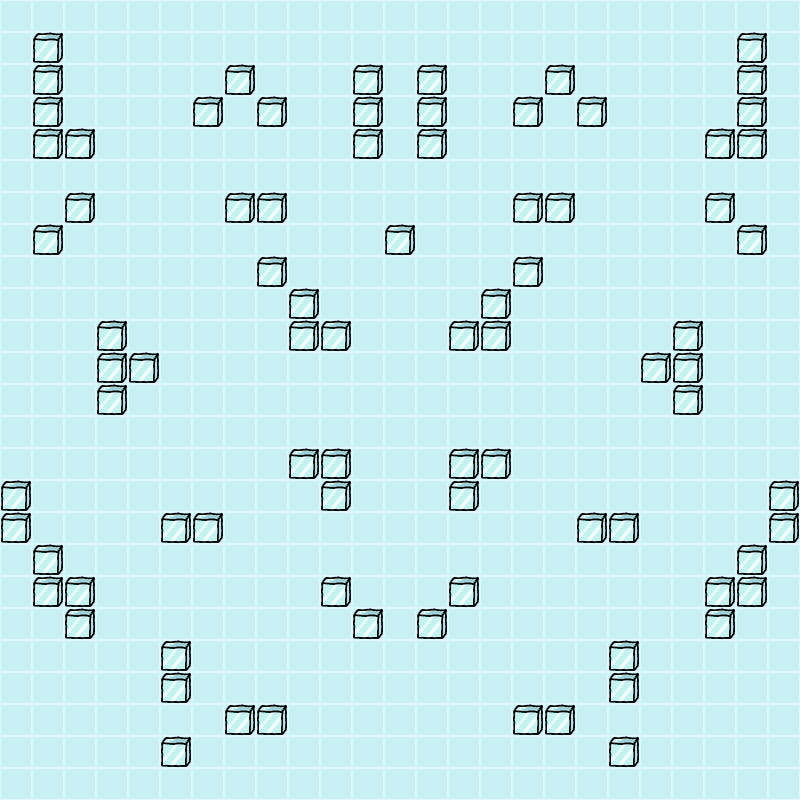
\includegraphics[width=0.65\textwidth]{../img/map}
    \end{center}
\end{frame}

\begin{frame}
    \frametitle{Nos agents de terrain}
    \begin{center}
        
\includegraphics[width=0.7\textwidth]{../logofinale_inv}
    \end{center}
\end{frame}

\begin{frame}
    \frametitle{Nos agents de terrain}
    \begin{itemize}[<+->]
        \item Redoutables, parfaitement à l'aise sur la glace, mais...
        \item Totalement stupides
        \item Chaque recrue contrôle 4 agents
    \end{itemize}
\end{frame}

% FIXME: we do not see the differences enough
%\begin{frame}
%    \frametitle{"All your base are belong to us"}
%    \centering
%    \only<1>{\includegraphics[width=7cm]{../img/poster_prologin2018}}
%    \only<2>{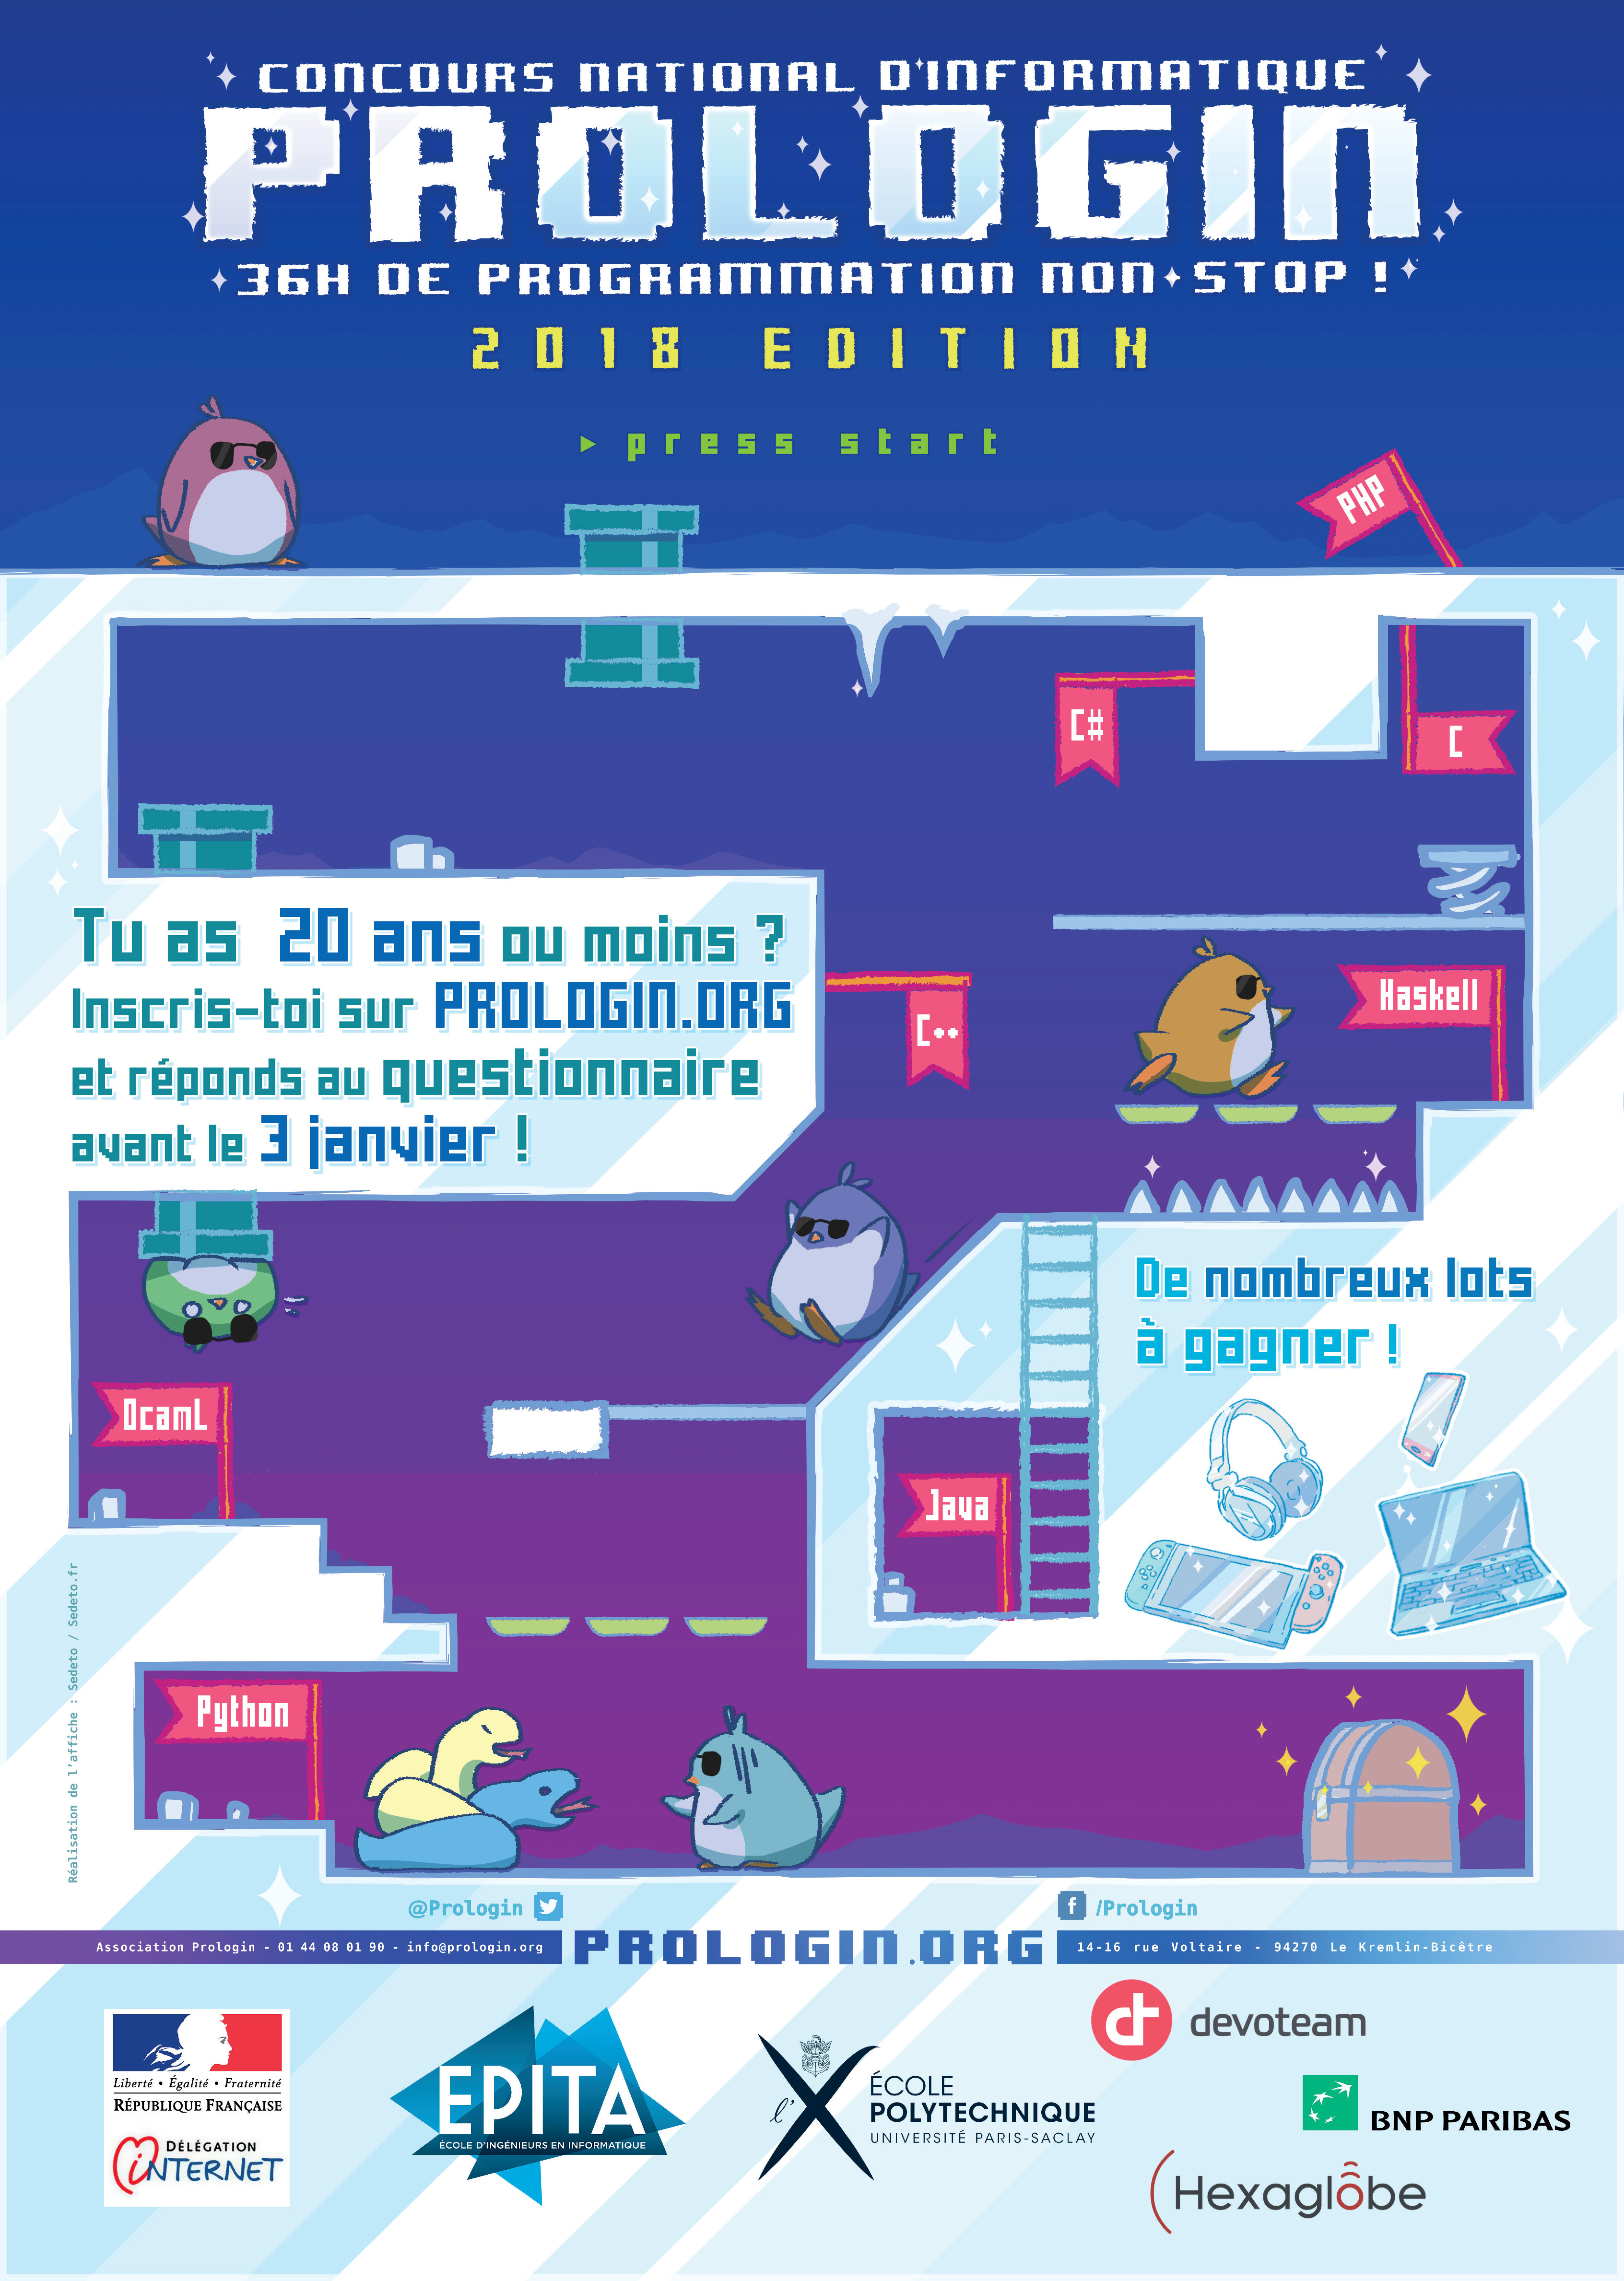
\includegraphics[width=7cm]{../img/poster_prologin2018_pib}}
%\end{frame}

\begin{frame}
    \frametitle{Aspects techniques}
    \begin{itemize}
        \item Simulation en tour par tour
        \item Objectif : capturer des aliens
        \item La mission dure 100 tours
    \end{itemize}
\end{frame}

\begin{frame}{Contrôle à distance}
    \begin{columns}[T]
    \begin{column}{0.3\textwidth}
        \begin{itemize}
            \item<1-> Déplacer
            \item<2-> Glisser
            \item<3-> Pousser
        \end{itemize}
    \end{column}
    \begin{column}{0.7\textwidth}
        \centering
        \only<1>{
            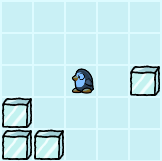
\includegraphics[width=4cm]{../img/move}
        }
        \only<2>{
            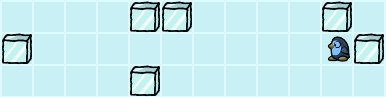
\includegraphics[width=7cm]{../img/slide1}
            \vspace{0.5cm}
            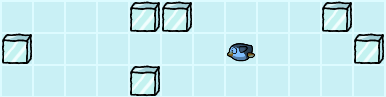
\includegraphics[width=7cm]{../img/slide2}
            \vspace{0.5cm}
            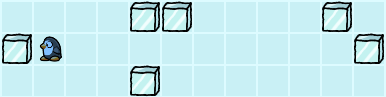
\includegraphics[width=7cm]{../img/slide3}
        }
        \only<3>{
            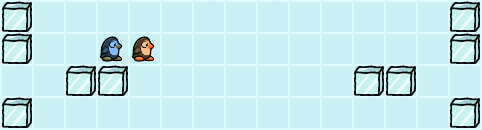
\includegraphics[width=7cm]{../img/push1}
            \vspace{0.3cm}
            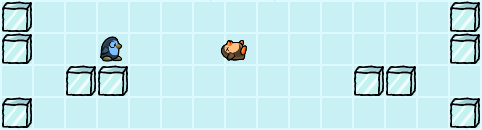
\includegraphics[width=7cm]{../img/push2}
            \vspace{0.3cm}
            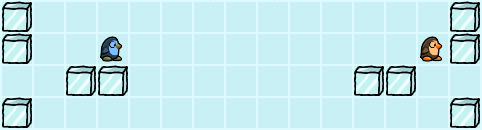
\includegraphics[width=7cm]{../img/push3}
        }
    \end{column}
    \end{columns}    
\end{frame}

\begin{frame}
    \frametitle{Aspects techniques}
    \begin{block}{Points d'action}
        \begin{itemize}
            \item À chaque tour, tous les agents ont 8 points d'action
            \item Les points ne sont utilisables que pour le tour actuel
            \item Pas de transfert de points entre agents
        \end{itemize}
    \end{block}
    \begin{block}{Coût}
        \begin{itemize}
            \item Déplacer : 1 point
            \item Glisser : 3 points
            \item Pousser : 5 points
        \end{itemize}
    \end{block}
\end{frame}

\begin{frame}
    \frametitle{Les aliens}
    \begin{columns}[T]
        \begin{column}{.2\textwidth}
            
\includegraphics[width=2.5cm]{../img/alien_big}
        \end{column}
        \begin{column}{.8\textwidth}
            \begin{itemize}
                \item Envahissent l'iceberg durant un certain nombre de tours
                \item Fixes par rapport à leur lieux d'invasion
                \item Ne sont \textbf{pas} des obstacles !
            \end{itemize}
            \only<2>{
                \vspace{1cm}
                \hspace{-2.5cm}
                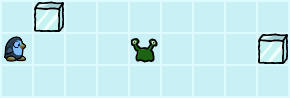
\includegraphics[width=5cm]{../img/alien_not_obstacle1}
                \hspace{0.5cm}
                
\includegraphics[width=5cm]{../img/alien_not_obstacle2}
            }
        \end{column}
    \end{columns}
\end{frame}

\begin{frame}
    \frametitle{Capture d'aliens}
    \begin{columns}[T]
    \begin{column}{0.5\textwidth}
        \begin{itemize}
            \item L'agent doit rester 3 tours sur la case de l'alien
            \item Si l'agent bouge de la case, la capture reprend \textbf{depuis 0}
            \item Une fois capturé, l'agent peut continuer sa mission tout de suite
            \item Chaque alien a un score attribué
        \end{itemize}
    \end{column}
    \begin{column}{0.5\textwidth}
        \centering
        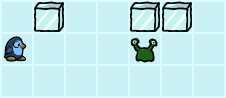
\includegraphics[width=4.5cm]{../img/alien_capture1}
        \vspace{0.5cm}
        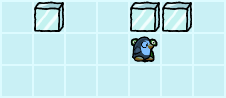
\includegraphics[width=4.5cm]{../img/alien_capture2}
        \vspace{0.5cm}
        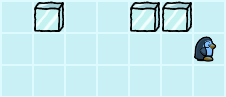
\includegraphics[width=4.5cm]{../img/alien_capture3}
    \end{column}
    \end{columns}    
\end{frame}

\begin{frame}
    \frametitle{Drapeaux de débug}
    \begin{columns}[T]
    \begin{column}{0.5\textwidth}
        \begin{itemize}
            \item Possibilité de placer des drapeaux sur n'importe quelles cases
            \item Trois types : rouge, vert, bleu
            \item Ne coûte pas de points d'action
        \end{itemize}
    \end{column}
    \begin{column}{0.5\textwidth}
        \centering
        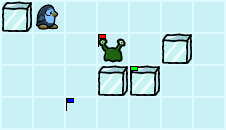
\includegraphics[width=5cm]{../img/debug_flags}
    \end{column}
    \end{columns}    
\end{frame}

\begin{frame}
    \frametitle{Exemple de simulation}
\end{frame}

\begin{frame}
    \frametitle{Questions}
    Posez vos questions sur le brief de mission !
\end{frame}

\begin{frame}
    \frametitle{Tournois intermédiaires}
    \begin{itemize}
        \item Samedi 15~h~42 (tournoi test)
        \item Samedi 17~h~42
        \item Samedi 23~h~42
        \item Dimanche 5~h~42
        \item Dimanche 11~h~42
        \item Dimanche 17~h~42
        \item Lundi 00~h~42 (tournoi final)
    \end{itemize}
\end{frame}

\begin{frame}
    \frametitle{Fin}
    Bonne chance pour votre mission...
    \pause

    ... mais d'abord, place à \textbf{l'importance vestimentaire}
\end{frame}

\end{document}
